\documentclass{article}
\usepackage{graphicx}
\usepackage{amsmath}
\usepackage{hyperref}
\usepackage{float}
\usepackage{xcolor}

\begin{document}

\title{Solutions to hw6 homework on Convex Optimization https://web.stanford.edu/class/ee364a/homework.html}
\author{Andrei Keino}
\maketitle

% Homework 6, due Friday 8/7/20:
% 7.7, 8.15, A13.2, A16.3, A18.2, A18.9.

% 7.7 p. 395
\section*{7.7}
ML estimation of Poisson distributions. Suppose $x_i,$ $i = 1, \dots , n$ are independent random variables with Poisson distributions 
$$
\boldsymbol{prob}(x_i = k) = \frac{e^{-\mu_i} \mu_i^k}{k!}
$$
with unknown means $\mu_i.$ The variables $x_i$ represent number of times that one of $n$ possible independent events occurs during a certain period. In emission tomography, for
example, they might represent the number of photons emitted by $n$ sources. We consider an experiment designed to determine the means $\mu_i.$ The experiment involves $m$ detectors. If event i occurs, it is detected by detector $j$ with probability $p_{ij}.$ We assume
the probabilities $p_{ij}$ are given (with $p{ij} \geq 0,$ 
$\sum_{j =1}^{m}p_{ij} \leq 1$). The total number of events
recorded by detector $j$ is denoted $y_j$,
$$
y_j = \sum_{i = 1}^{m} y_{ij}, \quad i = 1, \dots , m
$$

Formulate the ML estimation problem of estimating the means 
$\mu_i$ based on observed values of $y_j,$ $j = 1, \dots ,m,$ as
 a convex optimization problem.
 
 Hint: the variables $y_{ij}$ have the Poisson distribution with means $p_{ij} \mu_i, $ i.e 
$$
\boldsymbol{prob}(y_{ij} = k) = 
\frac{e^{-p_{ij}\mu_i} (p_{ij} \mu_i)^k}{k!}
$$
The sum of $n$ independent random variables with means 
$\lambda_1, \dots \lambda_n$ has a Poisson distribution with mean $\lambda_1 +  \dots + \lambda_n.$\\

Solution:

It follows from the hint, that 
$$
\boldsymbol{prob}(y_j = k) = 
\frac{e^{-p_j^T \mu} (p_j^T\mu)^k}{k!}
$$
Then likelihood of the set of $y_j = k_j,$ $j = 1, \dots , m$ is 

$$
L\{k_j\} = 
\prod_{j = 1}^{m}\frac{e^{-p_j^T \mu} (p_j^T\mu)^{k_j}}{k_j!}
$$
and the log likelihood is

$$
LL\{k_j\} = 
\sum_{j = 1}^{m}(-p_j^T \mu + k_j log(p_j^T\mu) - log(k_j!))
$$
$LL\{k_j\}$ is a concave function of $\mu_j.$ So, 
 the solution is:

\begin{align*}
\text{maximize } &
\sum_{j = 1}^{m}(-p_j^T \mu + k_j log(p_j^T\mu)) \\
\text{subject to } & \mu \succeq 0 \\
\end{align*} 

% 8.15 - p. 449
\section*{8.15}
Minimum volume ellipsoid covering union of ellipsoids.\\ Formulate the following problem
as a convex optimization problem. Find the minimum volume ellipsoid $\mathcal{E} = \{x \;| \; 
(x - x_0)^T A^{-1} (x - x_0) \leq 1\}$ that contains $K$ given ellipsoids 
$$
\mathcal{E}_i = \{x \;| \; (x)^T A_i x + 2b_i^Tx + c_i \leq 1\}
$$
Hint. See appendix \emph{{\color{red}B}}.\\
% appendix B - p. 653

Solution:\\ \\
$\mathcal{E}$ contains $\mathcal{E}_i$ if \\
$\forall x: \, x^T A^{-1} x - 2 x_0^T A^{-1} x + x_0^T A^{-1}x_0 - 1 \leq 0$ \\
$(x)^T A_i (x) + 2b_i^Tx + c_i - 1 \leq 0$\\
From the S - procedure in the appendix \emph{{\color{red}B}} we have it's true if there exists no such $\lambda \geq 0$ that:\\

$$
\lambda_i
\begin{bmatrix}
A_i& b_i\\
b_i^T & c_i
\end{bmatrix} -
\begin{bmatrix}
A^{-1} & -A^{-1}x_0\\
-(A^{-1}x_0)^T & x_0A^{-1}x_0 - 1\\
\end{bmatrix}
  \succeq 0
$$
this is the same as:

$$
\begin{bmatrix}
	\lambda_i A_i& \lambda_i b_i\\
	\lambda_i b_i^T & \lambda_i c_i + 1
\end{bmatrix} - 
\begin{bmatrix}
I\\
-x_0^T
\end{bmatrix} A^{-1} 
\begin{bmatrix}
I &
-x_0^T
\end{bmatrix}
\succeq 0
$$

So, we have SDP:

\begin{align*}
	\text{minimize } &log(det(A^{-1})) \\
	\text{subject to } &
	\begin{bmatrix}
		\lambda_i A_i&& \lambda_i b_i\\
		\lambda_i b_i^T && \lambda_i c_i + 1
	\end{bmatrix} - 
	\begin{bmatrix}
		I\\
		-x_0^T
	\end{bmatrix} A^{-1} 
	\begin{bmatrix}
		I &&
		-x_0^T
	\end{bmatrix}
	\succeq 0, \; i = 1, \dots, K\\
	& \lambda_i \geq 0, \; i = 1, \dots, K	
\end{align*} 

\section*{A13.2} % p. 148

Optimal spacecraft landing. We consider the problem of optimizing the thrust problem for a spacecraft
to carry out a landing at a target position. The spacecraft dynamics are
$$
m\ddot{p} = f - mge_3
$$
where $m > 0$ is the spacecraft mass, $p(t) \in R^3$ is the spacecraft position with 0 the target landing position and $p_3(t)$ representing height, 
$f(t) \in R^3$ is the thrust force and $g$ is the gravitational acceleration. (For simplicity we assume that the spacecraft mass is constant. This is not always
a good assumption, since the mass decreases with fuel use. We will also ignore any atmospheric
friction.) We must have $p(T^{td}) = 0$ and 
$\dot{p}(T^{td}) = 0$ where $T^{dt}$ is the touchdown time. The spacecraft must remain in a region given by
$$
p_3(t) \geq \alpha ||p_1(t), p_2(t)||_2
$$

where $\alpha > 0$ is a minimal given glide slope. The initial position $p(0)$ and velocity $\dot{p}(0)$ are given. The thrust force $f(t)$ is obtained from a single rocket engine on the spacecraft, with a given
maximum thrust; an attitude control system rotates the spacecraft to achieve any desired direction
of thrust. The thrust force is therefore characterized by the constraint $||f(t)||_2 \leq F^{max}.$ fuel
use rate is proportional to the thrust force magnitude, so the total fuel use is
$$
\int_{0}^{T^{td}} \gamma ||f(t)||_2 dt,
$$
where $\gamma > 0$ is the fuel consumption coefficient. The thrust force is discretized in time, i.e., it is
constant over consecutive time periods of length $h > 0$
with $f(t) = f_k$ for $t \in [(k - 1)h, kh]$ for 
$k = 1, \dots, K,$ where $T^{td} = Kh.$ Therefore we have:
\begin{align*}
v_{k + 1} &= v_{k} + (h / m) f_k- hge_3, \\
p_{k + 1} &= p_k + h / 2 (v_{k + 1} + v_k)
\end{align*} 
For simplicity, we will impose the glide slope constraint only at the times $t = 0, h, 2h, \dots, Kh.$\\

(a) Minimum fuel descent. Explain how to find the thrust profile $f_1, \dots, f_k$ that minimizes fuel
consumption, given the touchdown time $T^{td} = Kh$ and discretization time $h.$ \\

(b) Minimum time descent. Explain how to find the thrust profile that minimizes the touchdown time, i.e., $K,$ with $h$ fixed and given. Your method can involve solving several convex optimization problems. \\

(c) Carry out the methods described in parts (a) and (b) above on the problem instance with
data given in \verb!spacecraft_landing_data.*.!
Report the optimal total fuel consumption for
part (a), and the minimum touchdown time for part (b). The data files also contain plotting
code (commented out) to help you visualize your solution. Use the code to plot the spacecraft
trajectory and thrust profiles you obtained for parts (a) and (b).\\

Solution:

(a) To find the minimum fuel consumption profile 
we should minimize the expression 
$\sum_{k = 1}^K ||f_k||_2$. Then the problem is:

\begin{align*}
&\text{minimize} && \sum_{k = 1}^K ||f_k||_2\\ 
&\text{subject to} 
&&v_{k + 1} = v_{k} + (h / m) f_k- hge_3, \\
& &&p_{k + 1} = p_k + h / 2 (v_{k + 1} + v_k)\\
& && p_1 = p(0) \\
& && v_1 = \dot{p}(0)\\
& &&p_{K + 1} = 0 \\
& && v_{K + 1} = 0 \\
& && ||f_k||_2 \leq F^{max}, \; 
p_3(t) \geq \alpha ||p_1(t), p_2(t)||_2, 
\; k = 1, \dots, K\\
\end{align*} 
where $p_i, v_i, f_i, \; i = 1, \dots, K$ are variables.\\

(b) We can solve a sequence of convex feasibility problems tofind the minimum touchdown time. For each $K$ we solve the problem 

\begin{align*}
	&\text{minimize} && 0\\
	&\text{subject to} 
	&&v_{k + 1} = v_{k} + (h / m) f_k- hge_3, \\
	& &&p_{k + 1} = p_k + h / 2 (v_{k + 1} + v_k)\\
	& && p_1 = p(0) \\
	& && v_1 = \dot{p}(0)\\
	& &&p_{K + 1} = 0 \\
	& && v_{K + 1} = 0 \\
	& && ||f_k||_2 \leq F^{max}, \; 
	p_3(t) \geq \alpha ||p_1(t), p_2(t)||_2, 
	\; k = 1, \dots, K\\
\end{align*} 
where $p_i, v_i, f_i, \; i = 1, \dots, K$ are variables.\\
If the problem is feasible, we reduce $K$, otherwise we increase $K$. We iterate until we nd the smallest $K$ for which a feasible trajectory can be found.

(c) The matlab code:

\begin{verbatim}
spacecraft_landing_data;
% solve part (a) (find minimum fuel trajectory)
cvx_solver sdpt3;
cvx_begin
variables p(3,K+1) v(3,K+1) f(3,K)
v(:,2:K+1) == v(:,1:K)+(h/m)*f-h*g*repmat([0;0;1],1,K);
p(:,2:K+1) == p(:,1:K)+(h/2)*(v(:,1:K)+v(:,2:K+1));
p(:,1) == p0; v(:,1) == v0;
p(:,K+1) == 0; v(:,K+1) == 0;
p(3,:) >= alpha*norms(p(1:2,:));
norms(f) <= Fmax;
minimize(sum(norms(f)))
cvx_end
min_fuel = cvx_optval*gamma*h;
p_minf = p; v_minf = v; f_minf = f;
% solve part (b) (find minimum K)
% we will use a linear search, but bisection is faster
Ki = K;
while(1)
cvx_begin
variables p(3,Ki+1) v(3,Ki+1) f(3,Ki)
v(:,2:Ki+1) == v(:,1:Ki)+(h/m)*f-h*g*repmat([0;0;1],1,Ki);

p(:,2:Ki+1) == p(:,1:Ki)+(h/2)*(v(:,1:Ki)+v(:,2:Ki+1));
p(:,1) == p0; v(:,1) == v0;
p(:,Ki+1) == 0; v(:,Ki+1) == 0;
p(3,:) >= alpha*norms(p(1:2,:));
norms(f) <= Fmax;
minimize(sum(norms(f)))
cvx_end
if(strcmp(cvx_status,'Infeasible') == 1)
Kmin = Ki+1;
break;
end
Ki = Ki-1;
p_mink = p; v_mink = v; f_mink = f;
end
% plot the glide cone
x = linspace(-40,55,30); y = linspace(0,55,30);
[X,Y] = meshgrid(x,y);
Z = alpha*sqrt(X.^2+Y.^2);
figure; colormap autumn; surf(X,Y,Z);
axis([-40,55,0,55,0,105]);
grid on; hold on;
% plot minimum fuel trajectory for part (a)
plot3(p_minf(1,:),p_minf(2,:),p_minf(3,:),'b','linewidth',1.5);
quiver3(p_minf(1,1:K),p_minf(2,1:K),p_minf(3,1:K),...
f_minf(1,:),f_minf(2,:),f_minf(3,:),0.3,'k','linewidth',1.5);
print('-depsc','spacecraft_landing_a.eps');
% plot minimum time trajectory for part (b)
figure; colormap autumn; surf(X,Y,Z);
axis([-40,55,0,55,0,105]); grid on; hold on;
plot3(p_mink(1,:),p_mink(2,:),p_mink(3,:),'b','linewidth',1.5);
quiver3(p_mink(1,1:Kmin),p_mink(2,1:Kmin),p_mink(3,1:Kmin),...
f_mink(1,:),f_mink(2,:),f_mink(3,:),0.3,'k','linewidth',1.5);
print('-depsc','spacecraft_landing_b.eps');	
\end{verbatim}	

The optimal total fuel consumption is 193:0. The minimum touchdown
time is K = 25.


\section*{A16.3}

Utility versus latency trade-off in a network. We consider a network with $m$ edges, labeled $1, \dots m,$ and $n$ flows labeled $1, \dots, n.$ Each flow has an associated nonnegative flow rate $f_j;$ each edge or link has an associated positive capacity $c_i.$ Each flow passes over a fixed set of links (its route); the total traffic
$t_i$ on link $i$ is the sum of flow rates over all flows that pass though the link $i.$ The flow routes are described by a routing matrix 
$R \in \boldsymbol{R}^{m\times n},$ defined as:
$$
R_{ij} = 
\begin{cases}
	1 & \text{flow } j \text{ passes through link } i\\
	0 & \text{otherwise}\\
\end{cases}
$$

Thus, the vector fo link traffic, $t \in \boldsymbol{R}^m$ is given by $t = Rf.$ 
The link capacity constraint can be expressed as $Rf \preceq c.$ The logarithmic network utility is defined as $U(f) = \sum_{j = 1}^{n} log(f_j).$ The average queuing delay on link $i$ is given by 
$$
d_i = \frac{1}{c_i - t_i}
$$
multiplied by a constant that doesn't matter to us. We take $d_i = \infty$ for 
$t_i = c_i.$ The delay or latency for flow $j$ denoted $l_j$ is the sum of link delays
over all links that flow $j$ passes through. We define the maximum flow latency as
$$
L = max\{l_1, \dots l_n\}
$$
We are given $R$ and $c$, we are to choose $f.$\\

(a) How would you find the flow rates that maximize the utility $U$, ignoring 
flow latency? (In particular we allow $L = \infty.$) We'll refer to this maximum achievable utility as $U^{max}.$\\

(b) How would you find the flow rates that the maximum flow latency $L,$ ignoring utility? (In particular we allow $U = -\infty.$) We'll refer to this minimum achievable latency as $L^{min}.$ \\

(c) Explain how to find the optimal trade-off between utility $U$ (which we want to maximize) and latency $L$ (which we want to minimize). \\

(d) Find $U^{max}$, $L^{min}$ and plot the optimal trade-off utility versus latency 
for the network with the data given in  \verb!net_util_data.m!, showing $L^{min}$ 
and $U^{max}$ on the same plot. Your plot should cover the range from 
$L = 1.1 L^{min}$ to $L = 11 L^{min}.$ Plot $U$ vertically using linear scale and 
L horizontally using log scale. \\ 

Note. For parts (a), (b), and (c), your answer can involve solving one or more convex optimization problems. But if there is a simpler solution, you should say so.
\\

Solution: \\

(a) To maximize utility we solve the convex problem:

\begin{align*}
	&\text{maximize } &&  \sum_{j = 1}^{n} log(f_j) \\
	&\text{subject to } && Rf \preceq c\\
\end{align*} 
with variable $f$ and the implicit constraint $f \succeq 0.$ \\

(b) Link delay is monotonically increased with traffic and minimizes with zero traffic. Since flow latency is the sum of link delays, we can minimize the latency by setting the $f = 0.$ With $f = 0$ we have $d_i = 1 / c_i.$ To sum these delays over the routes, we multiply $d_i$ by $R^T.$ Then $l = R^T (1/c_1, \dots, 1/c_n),$
where $l$ is a vector of flow latencies. So, we have:
$$
L^{min} = max\{R^T (1/c_1, \dots, 1/c_n)\}
$$
where the $ max\{R^T (1/c_1, \dots, 1/c_n)\}$ is the maximum over the entries of the vector $R^T (1/c_1, \dots, 1/c_n).$\\


{c} Let $b_1, \dots b_m$ denotes the rows of R. To find the optimal trade - off between U and L we solve the problem 

\begin{align*}
	&\text{maximize } &&  \sum_{j = 1}^{n} log(f_j) \\
	&\text{subject to } && Rf \preceq c\\
	& && \sum_{i = 1}^m \frac{R_{ij}}{c_i - b_i^T f} \leq L, \; j = 1,\dots, n,
\end{align*} 
for a range of values $L.$ The variable here is $f$ and there is an implicit constraint $f \succeq 0.$ As $Rf \preceq c,$ we should have 
$c_i - b_i^T f \geq 0,$
so the constraints 
$$\sum_{i = 1}^m \frac{R_{ij}}{c_i - b_i^T f} \leq L$$
are convex (it can be easy verified considering the Hessian of \\
$\frac{R_{ij}}{c_i - b_i^T f}$ with variable $f.$ This is therefore a convex optimization problem.

% https://www.latex-tutorial.com/tutorials/figures/
\begin{figure}[H]
	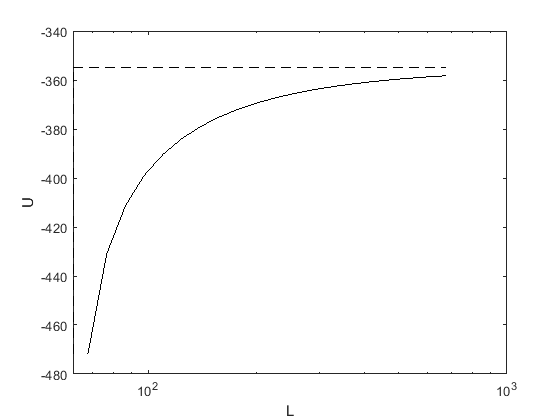
\includegraphics[width=\linewidth]{A16_3_plot.png}
	\caption{Optimal trade-off utility versus latency for the network.}
	\label{fig:A16_3_plot}
\end{figure}

The Matlab code:
\begin{verbatim}
% solution for network utility problem
clear all;
net_util_data;
% let's find max utility with no delay constraint
cvx_begin
variable f(n)
maximize geo_mean(f)
subject to
R*f <= c
f >= 0 % not needed; enforced by geomean domain
cvx_end
Umax=sum(log(f));

% let's find min latency with no utility constraint
% can be done analytically: just take f=0
Lmin = max(R'*(1./c));
% now let's do pareto curve
N = 20;
ds = 1.10*Lmin*logspace(0,1,N); % go from 10% above L
Uopt = [];
for d = ds
cvx_begin
variable f(n)
maximize geo_mean(f);
subject to
R'*inv_pos(c-R*f) <= d*ones(n,1)
f >= 0; % not needed; enforced by geomean domain
R*f <= c; % not needed; enforced by inv_pos domain
cvx_end
Uopt = [Uopt n*log(cvx_optval)];
end
semilogx(ds,Uopt,'k-',[Lmin,ds],[Umax,ones(1,N)*Umax],...
'k--',[1,1]*Lmin,[Uopt(1),Umax],'k--')
% axis([ds(1), ds(N), -480, -340]);
xlabel('L'); ylabel('U');	
\end{verbatim}	

\section*{A18.2}

Radiation treatment planning. In radiation treatment, radiation is delivered to a patient, with the
goal of killing or damaging the cells in a tumor, while carrying out minimal damage to other tissue.
The radiation is delivered in beams, each of which has a known pattern; the level of each beam can
be adjusted. (In most cases multiple beams are delivered at the same time, in one `shot', with the
treatment organized as a sequence of `shots'.) We let $b_j$ denote the level of beam $j,$ for $j = 1,\dots,n.$
These must satisfy $0 \leq b_j \leq B^{max},$ where $B^{max}$ is the maximum possible beam level. The exposure
area is divided into m voxels, labeled $i = 1,\dots,m.$ The dose $d_i$ delivered to voxel $i$ is linear in the beam levels, i. e., $d_j = \sum_{j=1}^n A_{ij}b_j.$
Here $A \in R_{+}^{m \times n}.$ is a (known) matrix
that characterizes the beam patterns. We now describe a simple radiation treatment planning problem. A (known) subset of the voxels, $\mathcal{T} \subset {1,\dots ,m}$
corresponds to the tumor or target region. We
require that a minimum radiation dose $D^{target}$ be administered to each tumor voxel, i.e., 
$d_i \geq D^{target}$ for $i \in \mathcal{T}.$ For all other voxels, we would like to have $d_i \leq D^{other},$ 
where $D^{other}$ is a desired maximum dose for non-target voxels. This is generally not feasible, so instead we settle for minimizing the penalty
$$
E = \sum_{i \notin \mathcal{T}}((d_i - D^{other})_{+})^2
$$

where $(\cdot)_+$ denotes the nonnegatie part. We can interpret $E$ as the sum of the squares of the
nontarget excess doses. \\

(a) Show that the treatment planning problem is convex. The optimization variable is $b \in R^n;$ the problem data are $A,$ $D^{other},$ $D^{target},$ $\mathcal{T},$
$B^{max}.$ \\

(b) Solve the problem instance with data given in the file \verb!treatment_planning_data.m!. Here we
have split the matrix $A$ into $Atarget$, which contains the rows corresponding to the target
voxels, and $Aother$, which contains the rows corresponding to other voxels. Give the optimal
value. Plot the dose histogram for the target voxels, and also for the other voxels. Make a
brief comment on what you see. Remark. The beam pattern matrix in this problem instance
is randomly generated, but similar results would be obtained with realistic data.\\

Solution:

(a) We have a problem:

\begin{align*}
	&\text{minimize } && \sum_{i \notin \mathcal{T}}(
	\sum_{j = 1}^{n} A_{ij}b_j - D^{other})_+^2\\
	&\text{subject to } && b_j \geq 0\\
	& && b_j \leq B^{max} \\
	& && \sum_{j = 1}^{n} A_{ij}b_j \geq D^{target}, 
	\; i \in  \mathcal{T} \\
\end{align*} 

function $(\cdot)_+$ is convex, its 
square is also convex, its argument is linear, so the whole minimized function is convex. The constraints are linear, so the problem is convex.\\

(b) \\
The matlab code:
\begin{verbatim}
% radiation treatment planning
treatment_planning_data;
cvx_begin
variable b(n); % beam intensities
minimize (sum(square_pos(Aother*b-Dother))) % minimize square excess dose delivered to others
subject to 
0 <= b;
b <= Bmax;
Atarget*b >= Dtarget % deliver minimum does to tumor voxels
cvx_end

subplot(2,1,1);
hist(Atarget*b);
axis([0 2 0 60]);
hold on; plot([Dtarget Dtarget],[0 60],'r')
title('Tumor voxel dose histogram')
subplot(2,1,2);
hist(Aother*b);
axis([0 2 0 150]);
hold on; plot([Dother Dother],[0 150],'r')
title('Other voxel dose histogram')
xlabel('Dosage')
print -depsc dose_histos	
\end{verbatim}	

\begin{figure}[H]
	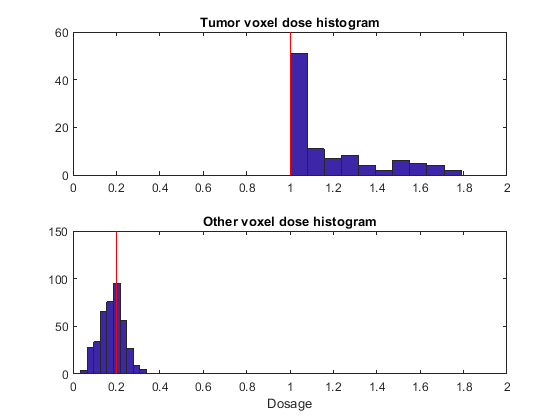
\includegraphics[width=\linewidth]{A_18_2_plot.png}
	\caption{The dose histogram, the vertical red lines corresponds to $D^{target}$ (top subplot) and $D^{other}$ (bottom subplot)}
	\label{fig:A_18_2_plot}
\end{figure}

\section*{A18.9}

Resource allocation in stream processing. A large data center is used to handle a stream of $J$ types of jobs. The traffic (number of instances per second) of each job type is denoted $t \in R_+^J.$ Each
instance of each job type (serially) invokes or calls a set of processes. There are $P$ types of processes, and we describe the job-process relation by the $P \times J$ matrix

$$
R_{pj} = 
\begin{cases}
	1, & \text{job} $j$ \text{invokes process} p \\
	0, & \text{otherwise}
\end{cases}
$$
The process loads (number of instances per second) are given by $\lambda = Rt \in R^P,$ i.e the $\lambda_p $ is the sum of the traffic from the jobs that invoke process $p.$
The latency of a process or job type is the average time that it takes one instance to complete. These are denoted 
$l^{proc} \in R^P$ and $l^{lob} \ in R^J$ respectfully
and are related by $l^{job} = R^T l^{proc},$ i.e $l_j^{job}$ is the sum of the latencies of the processes called by $j$. Job latency is important to users, since $L_j^{job}$ is the average time the data center takes to handle an instance of job type $j$. We are given a maximum allowed job latency:
$l^{job} \preceq l^{max}.$ The process latencies depend on the process load and also how much of n different resources are made available to them. These resources might include, for example, number of cores, disk storage,
and network bandwidth. Here, we represent amounts of these resources as (nonnegative) real
numbers, so $x_p \in R^n_+$ represents the resources allocated to process $p$. The process latencies are
given by
$$
l_p^{proc} = \psi_p(x_p, \lambda_p), \; p = 1, \dots, P,
$$
where $\psi_p: R^n\times R \leftarrow R \cup \{\infty\}$ is a known (extended-valued) convex function. These functions are
nonincreasing in their first (vector) arguments, and nondecreasing in their second arguments (i.e., more resources or less load cannot increase latency). We interpret
$\psi_p(x_p, \lambda_p) = \infty$ to mean that
the resources given by 
$x_p$ are not sufficient to handle
the load $\lambda_p.$ \\
We wish to allocate a total resource amount $x^{tot} \in R^n_{++}$ ampng the $p$ processes, so we have 
$\sum_{p = 1}^P x_p \preceq x^{tot}.$ The goal is to minimize the objective function
$$
\sum_{j = 1}^J w_j (t^{tar}_j - t_j)_+,
$$
where $(t^{tar}_j$ is the target traffic level for job type 
$j,$  $w_j > 0$ give the priorities, and $(u)_+$ is a
nonegative part of the vector, i.e 
${(u_i)}_+ = max\{u_i, 0\}.$ (Thus the objective is a weighted penalty for missing the target job traffic.) The variables are $t \in R_+^J$ and $x_p \in R_+^n,$ 
$p = 1, \dots, P.$ The problem data are matrix $R,$ the vectors $l^{max},$ $x^{tot},$ $t^{tar},$ and $w,$ and the functions $\psi_p, $ $p = 1, \dots, P.$ \\

(a) Explain why this is a convex optimization problem.\\


(b) Solve the problem instance with data given in \verb|res_alloc_stream_data.m|, with latency functions 
$$
\psi_p(x_p, \lambda_p) = 
\begin{cases}
	1 / (a_p^T x_p - \lambda_p), & a_p^T x_p > \lambda_p,  
	x_p \succeq x_p^{min} \\
	\\
	\infty, & \text{otherwise}
\end{cases}
$$
where $a_p \text{ and }x_p^{min}\in R^n{++}$ are given data.
The vectors $a_p$ and $x_p^{min}$ are stored as the columns of the matrices \verb|A| and \verb|x_min| respectfully.
Give the optimal objective value and job traffic. Compare the optimal job traffic with the target job traffic.\\


Solution:\\

(a) We have a task

\begin{align*}
	&\text{minimize } && 
	\sum_{j = 1}^J w_j (t^{tar}_j - t_j)_+\\
	&\text{subject to } 
	&& \sum_p x_p \leq x^{tot}, \; p = 1, \dots, P\\
	& && t \succeq 0\\
	& && \lambda = Rt\\
	& && l^{job} = R^T l^{proc}\\
	& && l^{job} \preceq l^{max}
\end{align*} 

with variables $x_p$ and $t,$ where 
$l^{proc} = \psi_p(x_p, \lambda_p).$
The  $\psi_p(x_p, \lambda_p)$ is convex, so the objective function is convex as a sum of convex functions. All the constraints are convex also.

(b) The Matlab code:

\begin{verbatim}	
res_alloc_stream_data;
% solution
cvx_begin
variable x(n,P) % resource allocation
variable t(J) % job traffic

minimize (w'*pos(t_tar-t))
subject to 
t >= 0
sum(x') <= x_tot'; % resource limits
lambda = R*t; % process loads
x >= x_min % minimum allowable resources for the processes
lproc = inv_pos(sum(A.*x)-lambda')'; % process latencies
ljob = R'*lproc; % job latencies
ljob <= l_max; % job latency limit
cvx_end
cvx_optval
[t t_tar]
[ljob l_max]	
\end{verbatim}	

The optimal objective value 7.7420.

The optimal objective value vs job traffic.
\begin{verbatim}	
9.0300    9.0300
8.5631    8.5631
6.8426    6.8426
1.6032    8.6306
6.3854    6.3854
9.9212    9.9212
9.3040    9.3040
5.9270    5.9270
2.0905    2.0905
2.8096    2.8096	
\end{verbatim}	


The latency of job vs its maximum latency allowed.
\begin{verbatim}	
1.1632    1.1632
1.5336    2.5734
1.4340    1.4340
1.8774    1.8774
1.8713    2.6975
0.8847    1.7482
1.6542    2.3063
1.7115    1.7115
2.0881    2.4848
2.3424    2.3424
\end{verbatim}	

\end{document}

